\chapter{Inteligência artificial}\label{cap:ia} % ou aprendizado de máquina?
\section{Introdução}\label{sec:ia_intro}
A inteligência artificial é um amplo ramo que trata de sistemas capazes de aprender e interpretar informações, e usar esse aprendizado para objetivos específicos.
%TODO: citação haenlein
Um dos campos da inteligência artificial é o aprendizado de máquina, onde a unidade de computação aprende a performar uma tarefa a partir de um conjuntos de exemplos de treinamento,
%TODO: citação louridas
funcionando como um tipo de modelo computacional do cérebro. Esses modelos são construídos a partir da interconexão entre unidades de processamento, por vezes chamados de neurônios artificiais, e por isso são conhecidas como \textbf{redes neurais artificiais}.

O tipo mais comum de aprendizado de máquina é o chamado \textbf{aprendizado supervisionado}, onde o modelo é apresentado a um conjunto de dados de exemplo que são rotulados, ou seja, cada entrada tem a sua saída definida. Durante o aprendizado, o modelo fornece uma saída e, a partir da saída verdadeira, ele se ajusta internamente para se aproximar mais do real.
%TODO: citação lecun
Quando não há uma saída real rotulada disponível, pode-se utilizar o \textbf{aprendizado não-supervisionado}. Nesse caso, o modelo tenta aprender alguns padrões nos dados, como grupos de exemplos similares. O aprendizado não-supervisionado tem a capacidade de identificar novos tipos de informações, já que não estão restritos aos rótulos.
%TODO: citacao aniscar

Os algoritmos de aprendizado de máquina também podem ser divididos quanto à atividade a ser realizada. Atividades de \textbf{classificação} identificam a classe da informação (por exemplo, se um animal é um cão ou gato) a partir de dados rotulados, o \textbf{agrupamento} (\textit{clustering}, em inglês) determina classes agrupando informações similares em grupos (\textit{clusters}) rotulados (como o agrupamento de filmes em gêneros), a \textbf{regressão} é usada para prever algum valor ou quantidade (como o preço de ações ao longo do tempo), e a \textbf{redução de dimensionalidade} representa dados de várias dimensões em outras menores (como as várias informações de um paciente sendo reduzidas às mais importantes para o diagnóstico de uma doença).

\section{Redes neurais}\label{sec:redesneurais}
O primeiro modelo de neurônio artificial foi o de McCulloch-Pitts, baseado em lógica binária e que possuía duas fase, a primeira onde o neurônio soma as contribuições de todos os neurônios anteriores, e a segunda onde o neurônio dispara apenas se um limiar for ultrapassado e não houver disparo de neurônio inibitório.
%TODO: citação mcculloch
Apesar de revolucionário para a época, um dos principais problemas do modelo de McCulloch-Pitts era a ausência do ajuste de pesos, ou seja, as conexões entre os neurônios sempre tinham a mesma força. Muitas pesquisas se desenvolveram na área para suprir essa necessidade, até que Frank Rosenblatt, inspirado pela teoria de Hebb vista anteriormente, criou o \textit{Perceptron},
%TODO: citacao rosenblatt
desenvolvido para ser um neurônio mais generalizado, sendo a base do aprendizado de máquina moderno. Matematicamente, o \textit{Perceptron} pode ser modelado pela seguinte equação:
\begin{equation}\label{eq:perceptron}
	y=\sigma\Big(\sum_{k=1}^Nw_kx_k+b\Big)
\end{equation}
onde $x_k$ é a resposta da sinapse $k$, $w_k$ é o peso da sinapse, $b$ é o \textit{bias} (viés, em português), um peso de referência que representa um conhecimento a priori, %TODO: elaborar
$\sigma$ é uma função de ativação não-linear, e $y$ é a saída do neurônio, como representado na Figura~\ref{fig:perceptron}. Resolvido o problema da atualização dos pesos, o \textit{Perceptron} sozinho é incapaz de realizar tarefas de separação não-linear,
%TODO: citação minsky
levando à criação, muitos anos depois, do \textit{Perceptron} de multi-camadas (MLP, \textit{Multilayer perceptron}, em inglês), que supre as limitações do \textit{Perceptron} simples ao agrupar camadas de neurônios, como na Figura~\ref{fig:mlp}. As camadas presentes entre a entrada e a saída da rede são chamadas de camadas ocultas (ou intermediárias).
\begin{figure}
	\centering
	\caption{Arquiteturas do Perceptron}
	\label{fig:perceptrons}
	\begin{subfigure}[b]{0.3\textwidth}
		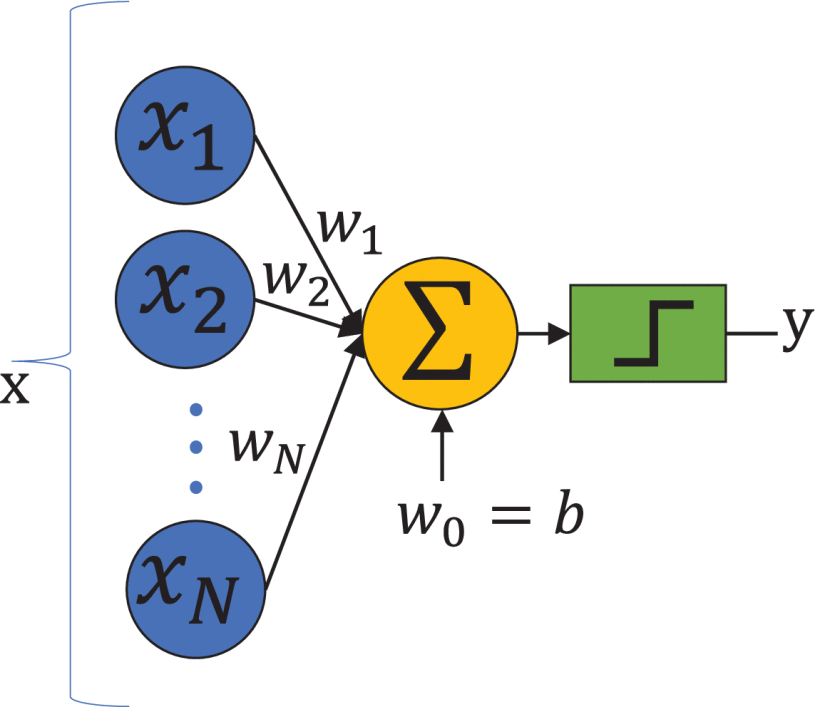
\includegraphics[width=\textwidth]{figs/perceptron}
		\caption{Perceptron}
		\label{fig:perceptron}
	\end{subfigure}
	\qquad\qquad
	\begin{subfigure}[b]{0.3\textwidth}
		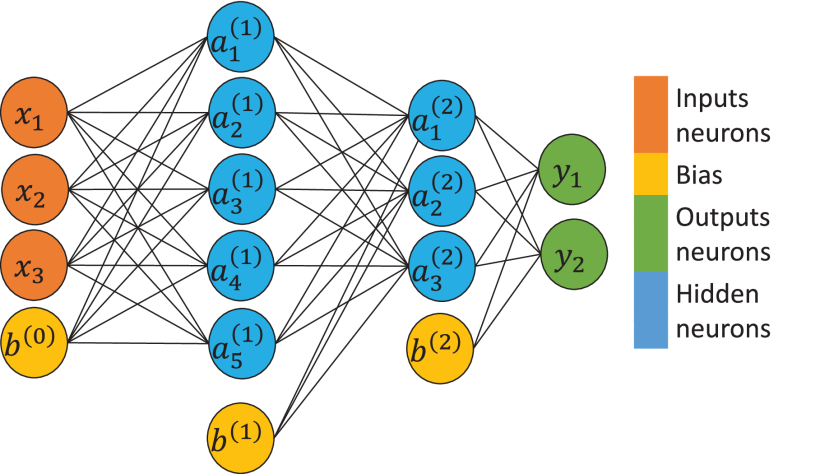
\includegraphics[width=\textwidth]{figs/mlp}
		\caption{Perceptron de multi-camadas}
		\label{fig:mlp}
	\end{subfigure}
	%TODO: trocar figura
\end{figure}

Os vários neurônios presentes nessa arquitetura frequentemente têm seus pesos atualizados através do algoritmo de gradiente descendente, que busca minimizar o erro entre a saída obtida pela rede e a real (aprendizado supervisionado), e essa atualização é feita através da metodologia da retro-propagação (\textit{backpropagation}, em inglês), ou seja, as atualizações das camadas finais da rede são propagadas em direção às iniciais.
%TODO: citação werbos
Quando há uma grande quantidade de camadas na rede ela é chamada de rede neural profunda (\textit{deep neural network}, em inglês), permitindo um mapeamento de dados mais complexos, o que não seria muito eficiente em redes não profundas. Uma lista não exaustiva de arquiteturas, profundas ou não, de redes neurais artificiais (\textit{artificial neural networks} (ANN), em inglês) é apresentada abaixo:
\begin{alineas}
	\item \textbf{\textit{Convolutional Neural Networks} (CNN, Redes neurais convolucionais)}: possui camadas que implementam a operação matemática de convolução, aplicando um filtro no sinal, e camadas de sub-amostragem (\textit{downsampling}), chamadas de \textit{pooling}. Essas redes lidam bem com sinais em duas dimensões, e por isso são frequentemente aplicadas em tarefas de visão computacional (relacionadas a imagens e vídeos);
	%TODO: citação lecun gradiente
	\item \textbf{\textit{Recurrent Neural Networks} (RNN, Redes neurais recorrentes)}: muito usadas em tarefas de entradas sequenciais, como processamento de fala e linguagem, possem a característica de processar os dados elemento a elemento, considerando também informações dos elementos passados, armazenados em pesos de conexões recorrentes, que funcionam como uma memória dinâmica para a rede;
	%TODO: citação elman finding
	\item \textbf{\textit{Hopfield Networks} (Redes Hopfield)}: proposta por J. J. Hopfield, são redes que são treinadas para aprender padrões (memórias) dos dados de maneira associativa, baseado no princípio de Hebb de que neurônios que disparam juntos se conectam;
	%TODO: citação hopfield
	\item \textbf{\textit{Autoencoder} (auto codificador)}: redes que aprendem a representar os dados reduzindo sua dimensionalidade, diminuindo as camadas ocultas, e, posteriormente, recriando os dados originais;
	%TODO: citação hinton reducing
	\item \textbf{\textit{Long Short-Term Memory} (LSTM, memória longa de curto prazo)}: uma variação da RNN composta de 4~(quatro) blocos de memória, sendo um principal e os outros três, chamados de portões de entrada, esquecimento e saída, responsáveis por alterar o estado da célula como um todo.
	%TODO: citação hochreiter
	Devida à sua capacidade de reter informações de longo tempo em séries temporais, são muito usadas em sistemas de reconhecimento de voz;
\end{alineas}
Além das arquiteturas citadas acima, existem outras que são baseadas no princípio de funcionamento do neurônio, envolvendo, inclusive, alterações físicas dos equipamentos onde são implementadas. Essas redes são chamadas de \textbf{neuromórficas}, detalhadas na seção seguinte.

\section{Redes neuromórficas}\label{sec:redesneuromorficas}
A maioria das redes neurais convencionais, derivadas da MLP, são implementadas com base na arquitetura de computadores de Von Neumann, onde as unidades de memória e processamento ficam separadas.
%TODO: citação von neumann
Algumas características dessa arquitetura incluem a codificação da informação para sinais binários (0 e 1) e os programas escritos em instruções explícitas (algoritmos), que são computadas pelo processador e os dados são armazenados na memória, trafegando por um barramento que conecta os dois elementos.

As arquiteturas neuromórficas surgem como uma opção onde estrutura e funcionamento são mais semelhantes ao do cérebro, em especial os neurônios e sinapses.
%TODO: citação ivanov neuromorphic
As redes neurais desenvolvidas com base nos princípios dessa arquitetura são chamadas de \textbf{redes neurais de disparo}~(\textit{spiking neural networks}, SNN, em inglês), cuja arquitetura é mostrada na Figura~\ref{fig:snn}. Diferentemente da arquitetura de Von Neumann, a neuromórfica distribui o processamento e memória em conjunto nos elementos de neurônio e sinapses, respectivamente, evitando o tempo da transmissão de informação através do barramento entre memória e processador.
%TODO: citação indiveri memory
Outra diferença da arquitetura neuromórfica é que a informação é codificada, tanto espacial quanto temporalmente, em sequências de potenciais de ação.
%TODO: citação frenkel bottom-up
Além disso, os programas de computadores neuromórficos são definidos pela estrutura da rede neural e seus parâmetros.
%TODO: citação schuman oportunities
\begin{figure}[tb]
	\centering
	\caption[Arquitetura de redes neurais de disparo (SNN)]{Arquitetura de redes neurais de disparo (SNN)}
	\label{fig:snn}
	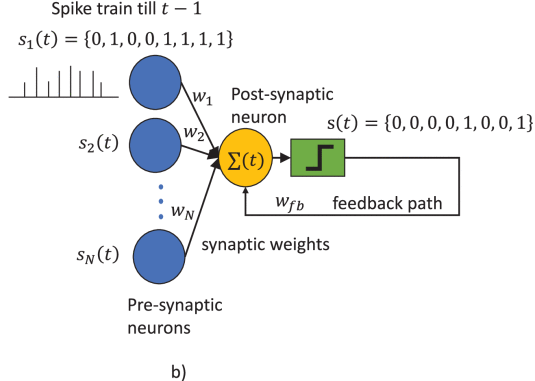
\includegraphics[width=0.7\linewidth]{figs/snn}
\end{figure}


Alguns projetos de dispositivos de \textit{hardware} foram desenvolvidos com base na arquitetura neuromórfica. O projeto \textbf{\textit{SpiNNaker}} propôs um computador paralelo massivo de milhões de núcleos, desenvolvido para a modelagem de redes neurais de disparo de grande escala.
%TODO: citação furber the spinnaker
O \textbf{\textit{BrainScaleS}} é um robusto sistema integrado de \textit{hardware} neuromórfico capaz de ser usado para modelar a complexidade neural, bem como topologias de rede realistas, permitindo a execução direta de modelos que anteriormente só eram possíveis de serem simulados numericamente.
%TODO: schemmel a wafer-scale
O projeto responsável pela sua criação, chamado de FACETS, participou do desenvolvimento do modelo AELIF, visto anteriormente, e esse modelo foi implementado fisicamente como um \textit{chip} presente no \textit{BrainScaleS}.
%TODO: aamir from lif to adex
O projeto \textbf{\textit{TrueNorth}} criou um chip com mais de 5~(cinco) bilhões de transistores e 4096~(quatro mil e noventa e seis) núcleos sinápticos, interconectados por uma rede de chips internos que integra 1~(um) milhão de neurônios de disparo programáveis e 256~(duzentas e cinquenta e seis) milhões de sinapses configuráveis.
%TODO: citação merolla a million spiking-neuron
O \textbf{\textit{Loihi}} é um chip de $60\ mm^2$ fabricado com processadores da Intel de $14-nm$ que integra uma variedade de recursos para o campo de redes neurais de disparo, como conectividade, compartimentos dendríticos, atrasos sinápticos e, mais importante, regras de aprendizado sinápticos programáveis.
%TODO: citação davies loihi

Diversos outros chips neuromórficos existem ou estão sendo pesquisados, com diferentes tecnologias de desenvolvimento e modelagem aplicadas,
%TODO: mehonic brain-inspired
alguns deles utilizando uma tecnologia chamada de \textbf{memristor}, uma espécie de transistor capaz de alterar a sua condutividade dependendo da corrente ou tensão aplicada aos seus terminais, sendo úteis para a implementação eficiente de computação em memória para as redes neurais de disparo.
%TODO: citação mehonic memristors
Vale destacar, também, que muitos desses dispositivos podem ser usados com redes neurais convencionais, como RNNs e CNNs, fazendo com que os estudos desse tipo de arquitetura estejam em alta.

As redes neurais de disparo usam, principalmente, neurônios do tipo integra-e-dispara para trocar informações via disparos de potencial de ação, e as unidades de computação são conectadas entre si e interagem através das sinapses.
%TODO: citação roy towards
É possível converter as redes neurais convencionais em redes de disparo fazendo alguns ajustes de pesos e normalização, a fim de tirar proveito das vantagens proporcionados pelo uso do \textit{hardware} neuromórfico.
%TODO: citação diehl conversion
Para fazer a conversão entre as redes neurais artificiais e as redes neurais de disparo, os dados de entrada precisam ser codificados em disparos de potencial de ação, e essa codificação pode ser baseada na taxa de disparo, na ordem de disparos de uma população, ou temporal.

Na codificação de taxa, a média temporal (quantidade de disparos por intervalo de tempo) ou a média de disparos de diferentes \textit{trials} é usada, tendo um correlato com o que ocorre em populações de neurônios do córtex auditivo primário.
%TODO: citação decharms primary
Na codificação de ordem de disparos de uma população vários neurônios diferentes disparam um potencial de ação, porém o importante não é o instante exato em que eles disparam, e sim a ordem deles, ou seja, qual neurônio disparou primeiro, qual foi o segundo, e assim por diante.
%TODO: citação mallot coding
A codificação temporal considera o exato momento em que ocorre o disparo do potencial de ação de cada neurônio, um comportamento neuronal de relevância.
%TODO: citação bohte the evidence
Subclassificações dessa codificação podem considerar apenas o instante do primeiro disparo ou a latência (a diferença de tempo entre os disparos). Os critérios para seleção do método de codificação variam por diferentes aspectos, como a minimização da perda de informação após a decodificação ou o aumento da acurácia de previsão/classificação.

Do ponto de vista do aprendizado das redes neurais de disparo, o não-supervisionado frequentemente faz uso da STDP como parte do seu mecanismo, com os pesos de potencialização e depressão de longa duração sendo atualizados durante o aprendizado.
%TODO: citação kheradpisheh stdp-based
No caso do aprendizado supervisionado, existe uma variação do método \textit{backpropagation}, relacionando as ativações das unidades de redes neurais com as taxas de disparo.
%TODO: citação diehl fast-classifying
No entanto, há discussões acerca do treinamento direto com \textit{backpropagation} na simulação do cérebro, principalmente na conversão de ANNs para SNNs. Algumas alternativas são encontradas na literatura, como o \textit{SpikeProp}, semelhante ao \textit{backpropagation},
%TODO: citação bohte error-backpropagation
o \textit{ReSuMe}, que pode ser usado em tarefas de tomada de decisão,
%TODO: citação ponulak supervised
e o \textit{SPAN}, que transforma as sequências de potenciais de ação na fase de treinamento em sinais analógicos, para que operações metemáticas comuns possam ser aplicadas.
%TODO: citação mohemmed span

% pensar onde colocar os simuladores
% \section{Simuladores neuronais}\label{sec:simuladores}
